
\documentclass[18pt,aspectratio=169]{beamer}
%\usetheme{kit}
\usepackage{ngerman}

% metropolis theme: https://github.com/matze/mtheme
\usetheme[sectionpage=progressbar,subsectionpage=progressbar,progressbar=frametitle]{metropolis}

% Notizen
%\setbeameroption{show notes}
%\setbeameroption{show notes on second screen=right}

\setbeamertemplate{section in toc}[sections numbered]
\setbeamertemplate{subsection in toc}[subsections numbered]

%redefine note page with bigger slide
\makeatletter
\defbeamertemplate*{note page}{mynotes}
{%
	{%
		\scriptsize
		\usebeamerfont{note title}\usebeamercolor[fg]{note title}%
		\ifbeamercolorempty[bg]{note title}{}{%
			\insertvrule{.45\paperheight}{note title.bg}%
			\vskip-.45\paperheight%
			\nointerlineskip%
		}%
		\vbox{
			\hfill\insertslideintonotes{0.45}\hskip-\Gm@rmargin\hskip0pt%
			\vskip-0.45\paperheight%
			\nointerlineskip
			\begin{pgfpicture}{0cm}{0cm}{0cm}{0cm}
				\begin{pgflowlevelscope}{\pgftransformrotate{90}}
					{\pgftransformshift{\pgfpoint{-2cm}{0.2cm}}%
						\pgftext[base,left]{\usebeamerfont{note date}\usebeamercolor[fg]{note date}\the\year-\ifnum\month<10\relax0\fi\the\month-\ifnum\day<10\relax0\fi\the\day}}
				\end{pgflowlevelscope}
		\end{pgfpicture}}
		\nointerlineskip
		\vbox to .45\paperheight{\vskip0.5em
			\hbox{\insertshorttitle[width=8cm]}%
			\setbox\beamer@tempbox=\hbox{\insertsection}%
			\hbox{\ifdim\wd\beamer@tempbox>1pt{\hskip4pt\raise3pt\hbox{\vrule
						width0.4pt height7pt\vrule width 9pt
						height0.4pt}}\hskip1pt\hbox{\begin{minipage}[t]{7.5cm}\def\breakhere{}\insertsection\end{minipage}}\fi%
			}%
			\setbox\beamer@tempbox=\hbox{\insertsubsection}%
			\hbox{\ifdim\wd\beamer@tempbox>1pt{\hskip17.4pt\raise3pt\hbox{\vrule
						width0.4pt height7pt\vrule width 9pt
						height0.4pt}}\hskip1pt\hbox{\begin{minipage}[t]{7.5cm}\def\breakhere{}\insertsubsection\end{minipage}}\fi%
			}%
			\setbox\beamer@tempbox=\hbox{\insertshortframetitle}%
			\hbox{\ifdim\wd\beamer@tempbox>1pt{\hskip30.8pt\raise3pt\hbox{\vrule
						width0.4pt height7pt\vrule width 9pt
						height0.4pt}}\hskip1pt\hbox{\insertshortframetitle[width=7cm]}\fi%
			}%
			\vfil}%
	}%
	\ifbeamercolorempty[bg]{note page}{}{%
		\nointerlineskip%
		\insertvrule{.55\paperheight}{note page.bg}%
		\vskip-.55\paperheight%
	}%
	\vskip.25em
	\nointerlineskip
	\insertnote
}
\makeatother

\setbeamertemplate{note page}[mynotes]

\makeatletter
\setbeamertemplate{section page}{
	\centering
	\begin{minipage}{22em}
		\raggedright
		\usebeamercolor[fg]{section title}
		\usebeamerfont{section title}
		\thesection.~\insertsectionhead\\[-1ex]
		\usebeamertemplate*{progress bar in section page}
		\par
		\ifx\insertsubsectionhead\@empty\else%
		\usebeamercolor[fg]{subsection title}%
		\usebeamerfont{subsection title}%
		\thesection.\thesubsection~\insertsubsectionhead
		\fi
	\end{minipage}
	\par
	\vspace{\baselineskip}
}
\makeatother

\definecolor{myColor}{HTML}{4477AA}
\definecolor{pitchblack}{HTML}{000000}
\setbeamercolor{alerted text}{fg=myColor}
\setbeamercolor{frametitle}{bg=pitchblack, fg=white}

\makeatletter
\setlength{\metropolis@titleseparator@linewidth}{1pt}
\setlength{\metropolis@progressonsectionpage@linewidth}{2pt}
\setlength{\metropolis@progressinheadfoot@linewidth}{2pt}
\makeatother


% uncomment the following line if you want to hide the navigation symbols
%\beamertemplatenavigationsymbolsempty 

\title{Automaten und Formale Sprachen}
\subtitle{Theoretische Informatik 1}
\author{\texorpdfstring{Peter Kossek\newline\href{mailto:e0030414@edu.dhsn.de}{\scriptsize e0030414@edu.dhsn.de}}{Peter Kossek}}

\institute{Duale Hochschule Sachsen, Studienakademie Leipzig} % Deutsch
\date{}

\makeatletter
\@addtoreset{figure}{section}
\@addtoreset{table}{section}
\makeatother

\renewcommand{\thefigure}{\thesection.\arabic{figure}}

\renewcommand{\thetable}{\thesection.\arabic{table}}

\usepackage{nameref}
\makeatletter
\newcommand*{\currentname}{\@currentlabelname}
\makeatother

\usepackage{circuitikz}
\usepackage{tikz}
\usetikzlibrary{automata, positioning, arrows}

%strikeout text in math mode
\usepackage[normalem]{ulem}
\usepackage{amsmath}
\newcommand{\stkout}[1]{\ifmmode\text{\sout{\ensuremath{#1}}}\else\sout{#1}\fi}

\usepackage{tabularx} %same-width columns
\newcolumntype{Y}{>{\centering\arraybackslash}X} %columntype Y is centered column for tabularx

\setcounter{tocdepth}{1} % only sections in TOC

\usepackage{wasysym} %for lightning symbol

\usepackage{qrcode} %for QR codes

\begin{document}

\selectlanguage{ngerman}

%title page
\begin{frame}
	\titlepage
\end{frame}

%\begin{frame}
%	\frametitle{Danksagung}
%	Diese Vorlesung basiert maßgeblich auf dem Script von\\
%	Prof. Dr. habil. Jochen Kripfganz\\
%	Dozent für Theoretische Informatik an der BA Leipzig bis 2021
%\end{frame}

\begin{frame}{Organisatorisches}
	\begin{itemize}
		\item Vorlesungen
		\item Übungen
		\item Fragen jeder Art
		\item besondere Bedürfnisse
	\end{itemize}
\end{frame}

\AtBeginSection{
	\begin{frame}
		\sectionpage
		\tableofcontents[sectionstyle=hide/hide,subsectionstyle=show/show/hide]
	\end{frame}
}

\begin{frame}
	\frametitle{Literatur}
	\begin{columns}
		\column{.8\textwidth}
			\begin{itemize}
				\item Script zur Vorlesung \\
				{\small \url{https://github.com/bluepoke/Automaten_Formale_Sprachen/releases/latest}}
				\item Grundlage der Vorlesung
				\begin{itemize}
					\item Schöning, U.: \textit{Logik für Informatiker}
					\item Schöning, U.: \textit{Theoretische Informatik - kurz gefasst}
				\end{itemize}
				\item Weitere Literatur
				\begin{itemize}
					\item Vossen, G.; Witt, K. U.: \textit{Grundlagen der Theoretischen Informatik mit Anwendungen}
					\item Hollas, B.: \textit{Grundkurs Theoretische Informatik}
					\item Erk, K.;  Priese, L.: \textit{Theoretische Informatik}
				\end{itemize}
			\end{itemize}
		\column{.2\textwidth}
				\qrcode[height=0.9\textwidth]{https://github.com/bluepoke/Automaten_Formale_Sprachen/releases/latest}
	\end{columns}
\end{frame}

%table of contents
\begin{frame}
	\frametitle{Gliederung}
	\tableofcontents
\end{frame}

\begin{frame}{Wozu brauche ich das?}
	
	$$L(A)=\left\{w \in \Sigma^* \mid w=0 \lor w=x00, x\in \Sigma^*\right\}$$
	
	\begin{align*}
		\delta = \{&(s_0, a, s_1, x, R), (s_0, x, s_0, x, R), (s_0, \#, s_f, \#, N),\\
		&(s_1, x, s_1, x, R), (s_1, a, s_1, a, R), (s_1, b, s_2, x, R),\\
		&(s_2, b, s_2, b, R), (s_2, \#, s_3, \#, L), (s_3, b, s_3, b, L),\\
		&(s_3, x, s_3, x, L), (s_3, a, s_3, a, L), (s_3, \#, s_0, \#, R)\}
	\end{align*}
\end{frame}

%\frame{
%	\frametitle{Sprachen im Kontext der Informatik}
%	
%	\begin{itemize}
%		\item \emph{Sprache:} Menge zulässiger Worte über einem Alphabet
%		\item \emph{Programm:} String über einem Alphabet von Eingabezeichen (Quellcode) bzw. binär über 0/1
%		\item \emph{Compiler:} 
%		\begin{itemize}
%			\item prüft die Zulässigkeit dieses Strings als Satz (Wort) einer Sprache
%			\item generiert Folge von Maschinenbefehlen
%		\end{itemize}
%		\item \emph{Lexikalische Analyse:} Übersetzer-Modul ("`Scanner"') fasst Symbolfolgen zu Schlüsselworten ("`Token"') zusammen
%		\item \emph{Syntaxanalyse:}
%		\begin{itemize}
%			\item "`Parser"' prüft, ob Folge von Token zulässig ist
%			\item Semantik-Prüfung erfolgt dabei nicht
%		\end{itemize}
%	\end{itemize}
%}

\section{Aussagenlogik}

\subsection{Aussagenlogische Formeln}

\begin{frame}{Syntax}
	\begin{itemize}
		\item \emph{Aussage:} Satz, der entweder wahr ($w$) oder falsch ($f$) ist; Aussagenvariable $A$; Wahrheitswert $w(A)$
		\item \emph{Syntax:} Induktive Definition korrekt gebildeter aussagenlogischer Formeln F über Variablenmenge $V=\{A, B, \ldots\}$:
		\begin{itemize}
			\item Die Booleschen Wahrheitswerte $w$ und $f$ sind Formeln
			\item Jede Variable aus $V$ ist eine Formel: \emph{Atome}
			\item Negation: $\neg F$ ist eine Formel
			\item Konjunktion: $(F_1 \land F_2)$ ist eine Formel
			\item Disjunktion: $(F_1 \lor F_2)$ ist eine Formel
			\item Implikation: $(F_1 \rightarrow F_2)$ ist eine Formel
			\item Äquivalenz: $(F_1 \leftrightarrow F_2)$ ist eine Formel
			\item andere Verknüpfungen bilden keine Formel
		\end{itemize}
	\end{itemize}
\end{frame}

\begin{frame}{Präzedenzregeln}
	Vereinbarung zur Reduzierung von Klammern
	\begin{itemize}
		\item Bindung (analog "`Punkt vor Strich"'-Rechnung)
		\begin{itemize}
			\item $\neg$ bindet stärker als $\land$
			\item $\land$ bindet stärker als $\lor$
			\item $\lor$ bindet stärker als $\rightarrow$ und $\leftrightarrow$
		\end{itemize}
		\item Operatoren gleicher Stärke: Auswertung linksassoziativ; z.B. \\ $(A \lor B \lor C)$ steht für $((A \lor B) \lor C)$
		\item äußere Klammer weglassen: $(((A \lor B) \rightarrow C) \land B) \mapsto (A \lor B \rightarrow C) \land B$
	\end{itemize}
\end{frame}

\begin{frame}{Semantik}
	aussagenlogischen Formeln wird eine Bedeutung zugeordnet
	\begin{itemize}
		\item Def. Belegung (Interpretation) $I: V \rightarrow \{f, w\}$\\ den Atomen wird jeweils ein konkreter Wahrheitswert zugeordnet
		\item schrittweise (über die Bewertung von Teilformeln) lassen sich dann zusammengesetzte Formeln bewerten:
		\begin{itemize}
			\item $I(\neg F)=w$ falls $I(F)=f$, sonst $I(\neg F)=f$
			\item $I(F \land G)=w$ falls $I(F)=w$ und $I(G)=w$, sonst $I(F \land G)=f$
			\item $I(F \lor G)=w$ falls $I(F)=w$ oder $I(G)=w$, sonst $I(F \lor G)=f$
			\item $I(F \rightarrow G)=w$ falls $I(F)=f$ oder $I(G)=w$, sonst $I(F \rightarrow G)=f$
			\item $I(F \leftrightarrow G)=w$ falls $I(F)=I(G)$, sonst $I(F \leftrightarrow G)=f$
		\end{itemize}
	\end{itemize}
\end{frame}

\begin{frame}{Semantik: Darstellung per Wahrheitstafel}
	Wahrheitstafel enthält zeilenweise alle möglichen Belegungen
	\begin{table}
		\centering
			\begin{tabular}{|c|c|c|c|c|c|c|}
				\hline
				$A$ & $B$ & $\neg A$ & $A \land B$ & $A \lor B$ & $A \rightarrow B$ & $A \leftrightarrow B$ \\
				\hline
				f & f & w & f & f & w & w \\
				\hline
				f & w & w & f & w & w & f \\
				\hline
				w & f & f & f & w & f & f \\
				\hline
				w & w & f & w & w & w & w \\
				\hline
			\end{tabular}
			\caption{Wahrheitstafel der Grundoperationen}
		\end{table}
		semantische Äquivalenz $F_1 \equiv F_2$: $F_1$ und $F_2$ haben gleichen Wahrheitswerteverlauf; z.B.\\
		$A \rightarrow B \equiv \neg A \lor B$\\
		$A \leftrightarrow B \equiv (A \rightarrow B) \land (B \rightarrow A)$
\end{frame}

\begin{frame}{Erfüllbarkeit, Tautologie, Kontradiktion}
	\begin{itemize}
		\item Sei $F$ eine Formel und $I$ eine Belegung. Falls $I$ für alle in $F$ vorkommenden Atome definiert ist, so heißt $I$ \underline{zu $F$ passend}
		\item Falls $I$ zu $F$ passend ist, und es gilt $I(F)=w$, dann heißt $I$ \underline{Modell für $F$}; Schreibweise: $I \models F$
		\item $F$ heißt \underline{erfüllbar}, falls $F$ mindestens ein Modell besitzt; sonst heißt $F$ \underline{unerfüllbar} (Kontradiktion; Schreibweise $F\bot$)
		\item $F$ heißt gültig bzw. \underline{Tautologie}, falls jede zu $F$ passende Belegung $I$ ein Modell für $F$ ist; Schreibweise $\models F$ oder $F\top$ \\
		Beispiel: $(A \land B) \rightarrow A$
		\item es gilt: $F$ ist Tautologie gdw. $\neg F$ ist Kontradiktion
	\end{itemize}
\end{frame}

\begin{frame}{Äquivalenz aussagenlogischer Formeln}
	\begin{itemize}
		\item Zwei Formeln $F$ und $G$ heißen semantisch äquivalent ($F \equiv G$), falls für alle Belegungen $I$ gilt: $I(F)=I(G)$
		\item Äquivalenz kann bewiesen (oder widerlegt) werden durch Aufstellen der jeweiligen Wahrheitstafeln
		\item Beispiele
		\begin{itemize}
			\item $A \rightarrow B \equiv \neg A \lor B$
			\item $A \leftrightarrow B \equiv (A \land B) \lor (\neg A \land \neg B) \equiv (A \rightarrow B) \land (B \rightarrow A)$
		\end{itemize}
		\item Ersetzbarkeitstheorem:\\
		enthält eine Formel $F$ eine Teilformel $G$ und wird $G$ durch eine äquivalente Formel ersetzt, so entsteht eine zu $F$ äquivalente Formel
	\end{itemize}
\end{frame}

\begin{frame}{Äquivalenzen als Rechenregeln}
	\begin{itemize}
		\item Idempotenz
		\begin{itemize}
			\item $(A \land A) \equiv A$
			\item $(A \lor A) \equiv A$
		\end{itemize}
		\item Kommutativgesetz
		\begin{itemize}
			\item $(A \land B) \equiv (B \land A)$
			\item $(A \lor B) \equiv (B \lor A)$
		\end{itemize}
		\item Assoziativgesetz
		\begin{itemize}
			\item $(A \land (B \land C)) \equiv ((A \land B) \land C)$
			\item $(A \lor (B \lor C)) \equiv ((A \lor B) \lor C)$
		\end{itemize}
		\item Distributivgesetz
		\begin{itemize}
			\item $(A \land (B \lor C)) \equiv ((A \land B) \lor (A \land C))$
			\item $(A \lor (B \land C)) \equiv ((A \lor B) \land (A \lor C))$
		\end{itemize}
	\end{itemize}
\end{frame}

\begin{frame}{Äquivalenzen als Rechenregeln (Fortsetzung)}
	\begin{itemize}
		\item Absorptionsgesetz
		\begin{itemize}
			\item $(A \land (A \lor B)) \equiv A$
			\item $(A \lor (A \land B)) \equiv A$
		\end{itemize}
		\item Doppelnegation
		\begin{itemize}
			\item $\neg \neg A \equiv A$
		\end{itemize}
		\item deMorgansche Regeln
		\begin{itemize}
			\item $\neg (A \land B) \equiv (\neg A \lor \neg B)$
			\item $\neg (A \lor B) \equiv (\neg A \land \neg B)$
		\end{itemize}
		\item Tautologieregeln: sei $A$ Tautologie; $A\top$ bzw. $\models A$ bzw. $A \equiv w$
		\begin{itemize}
			\item $(A \lor B) \equiv (w \lor B) \equiv w \equiv A$; $(A \land B) \equiv (w \land B) \equiv B$
		\end{itemize}
		\item Kontradiktionsregeln: sei $A$ Kontradiktion; $A\bot$ bzw. $A \equiv f$
		\begin{itemize}
			\item $(A \lor B) \equiv (f \lor B) \equiv B$; $(A \land B) \equiv (f \land B) \equiv f \equiv A$
		\end{itemize}
	\end{itemize}
\end{frame}

\begin{frame}{Beispiel: direkter Beweis der Gültigkeit einer Formel\\ \hspace{1.6cm} (als Alternative zur Wahrheitstafel)}
	\begin{columns}
		\column{.5\textwidth}
		\begin{eqnarray*}
				F &=& (A \land (A \rightarrow B)) \rightarrow B\\
				  &\equiv& \neg (A \land (A \rightarrow B)) \lor B\\
				  &\equiv& \neg (A \land (\neg A \lor B)) \lor B\\
				  &\equiv& \neg A \lor \neg(\neg A \lor B) \lor B\\
				  &\equiv& \neg A \lor (A \land \neg B) \lor B\\
				  &\equiv& \neg A \lor (A \lor B) \land (\neg B \lor B)\\
				  &\equiv& \neg A \lor (A \lor B) \land w\\
				  &\equiv& \neg A \lor A \lor B\\
				  &\equiv& w \lor B\\
				  &\equiv& w
		\end{eqnarray*}
		\column{.5\textwidth}
			\begin{tabular}{|c|c|c|c||c|}
				\hline
				$A$ & $B$ & $A \rightarrow B$ & $A \land (A \rightarrow B)$ & $F$ \\
				\hline
				f & f & w & f & w \\
				%\hline
				f & w & w & f & w \\
				%\hline
				w & f & f & f & w \\
				%\hline
				w & w & w & w & w \\
				\hline
			\end{tabular}
	\end{columns}		
\end{frame}

\begin{frame}{Normalformen}
	\begin{itemize}
		\item \emph{Literal:} Aussagenvariable $A$ ("`positives Literal"') oder negierte Aussagenvariable $\neg A$ ("`negatives Literal"')
		\item \emph{Negationsnormalform (NNF)}: Formel $F$ ist in NNF, falls $\rightarrow$ und $\leftrightarrow$ aufgelöst sind und alle Negationszeichen $\neg$ unmittelbar vor einer Aussagenvariable stehen.\\
		beachte: NNF ist nicht eindeutig
		\item \emph{Monom:} Konjunktion von Literalen, d.h. Formel der Art\\
		$\bigwedge_iL_i=L_1\land L_2\land\ldots\land L_k$
		\item \emph{Klausel:} Disjunktion von Literalen, d.h. Formel der Art\\
		$\bigvee_iL_i=L_1\lor L_2\lor\ldots\lor L_k$
	\end{itemize}
\end{frame}

\begin{frame}{Disjunktive Normalform (DNF) und Konjunktive Normalform (KNF)}
	\begin{itemize}
		\item Disjunktive Normalform \emph{DNF:} Disjunktion von Konjunktionen (Monomen)\\
		$F=\bigvee_i\left(\bigwedge_jL_{ij}\right)$
		\item Konjunktive Normalform \emph{KNF:} Konjunktion von Disjunktionen (Klauseln)\\
		$F=\bigwedge_i\left(\bigvee_jL_{ij}\right)$
		\item Für jede Formel existiert eine äquivalente Formel in KNF und eine äquivalente Formel in DNF
		\begin{itemize}
			\item Erzeuge NNF $\mapsto$ DNF bzw. KNF\\
			DNF: ersetze Ausdrücke der Art $(F \land (G \lor H))$ durch $(F \land G) \lor (F \land H)$ solange solche Teilformen existieren\\
			KNF: ersetze Ausdrücke der Art $(F \lor (G \land H))$ durch $(F \lor G) \land (F \lor H)$ solange solche Teilformeln existieren
		\end{itemize}
	\end{itemize}
\end{frame}

\note{
Beispiel DNF/KNF durch Umformung:
\begin{align*}
	\neg &(x \leftrightarrow y) \rightarrow z\\
  \equiv &(x \leftrightarrow y) \lor z\\
  \equiv &(x \land y) \lor (\neg x \land \neg y) \lor z \textrm{\qquad[DNF]}\\
  \equiv &(\underbrace{(x \lor \neg x)}_1 \land (x \lor \neg y) \land (y \lor \neg x) \land \underbrace{(y \lor \neg y)}_1) \lor z\\
  \equiv &((x \lor \neg y) \land (y \lor \neg x)) \lor z\\
  \equiv &(x \lor \neg y \lor z) \land (y \lor \neg x \lor z) \textrm{\qquad[KNF]}
\end{align*}

}

\begin{frame}{Konstruktion kanonische DNF/KNF aus Wahrheitstafel}
	\begin{itemize}
		\item \emph{Kanonische} DNF bzw. KNF: jede Aussagenvariable kommt in jedem Monom bzw. jeder Klausel genau einmal vor (positiv oder negativ)
		\item Kanonische NF lassen sich aus der Wahrheitstafel der Formel ablesen
		\begin{itemize}
			\item Kanonische DNF (KDNF)
			\begin{itemize}
				\item Je ein Monom für jede Belegung mit Wahrheitswert $w$
				\item Setze $L_j=A_j$, falls $w(A_j)=w$, $L_j=\neg A_j$ sonst
			\end{itemize}
			\item Kanonische KNF (KKNF)
			\begin{itemize}
				\item Je eine Klausel für jede Belegung mit Wahrheitswert $f$
				\item Setze $L_j=\neg A_j$, falls $w(A_j)=w$, $L_j=A_j$ sonst
			\end{itemize}
		\end{itemize}
		\item Übungsbeispiel (KNF, aber nicht kanonisch)\\
		$F=\neg B \land (A \lor \neg C)$
	\end{itemize}
\end{frame}

\begin{frame}{Beispiel: Konstruktion von KDNF und KKNF aus Wahrheitstafel}
	\begin{columns}
		\column{.3\textwidth}
		\begin{center}
			\begin{tabular}{|c|c|c||c|}
				\hline
				A & B & C & F \\
				\hline
				0 & 0 & 0 & 1 \\
				0 & 0 & 1 & 0 \\
				0 & 1 & 0 & 0 \\
				0 & 1 & 1 & 0 \\
				1 & 0 & 0 & 1 \\
				1 & 0 & 1 & 1 \\
				1 & 1 & 0 & 0 \\
				1 & 1 & 1 & 0 \\
				\hline
			\end{tabular}
		\end{center}
		\column{.7\textwidth}
		\begin{itemize}
			\item [KDNF:] Werte für F=1 auslesen
			$$(\neg A \land \neg B \land \neg C) \lor (A \land \neg B \land \neg C) \lor (A \land \neg B \land C)$$
			\item [KKNF:] Werte für F=0 auslesen und Literale negieren
			\begin{align*}
				&(A \lor B \lor \neg C) \land (A \lor \neg B \lor C) \land \\
				&(A \lor \neg B \lor \neg C) \land (\neg A \lor \neg B \lor C) \land (\neg A \lor \neg B \lor \neg C)
			\end{align*}
			\item Minimierung der KKNF und KDNF durch Karnaugh-Veitch-Diagramm möglich (dann aber i.d.R. nicht mehr kanonisch)
		\end{itemize}
	\end{columns}
\end{frame}

\begin{frame}{Beispiel: Karnaugh-Tafel}
	\begin{columns}
	\column{.5\textwidth}
	Karnaugh-Tafel für $F=\neg B \land (A \lor \neg C)$
	\begin{center}
		\begin{tabular}{|c||c|c|c|c|}
			\hline
			& $AB$ & $\neg A B$ & $\neg A \neg B$ & $A \neg B$ \\
			\hline
			\hline
			$C$ & 0 & 0 & 0 & 1 \\
			\hline
			$\neg C$ & 0 & 0 & 1 & 1 \\
			\hline
		\end{tabular}
	\end{center}
	\column{.5\textwidth}
	Abgeleitete Formeln:
	\begin{itemize}
		\item [DNF:] Einsen zu Blöcken (Größe $2^n$) und die Variablen im Block weglassen, die sowohl positiv als auch negativ vertreten sind. Variablen mit Konjunktion verknüpfen, Blöcke mit Disjunktion:\\
		$(\neg B \land \neg C) \lor (A \land \neg B)$
		\item [KNF:] Wie DNF, aber: Nullen zu Blöcken, Variablen negieren, Verknüpfungen umkehren\\
		$(\neg B) \land (A \lor \neg C)$
	\end{itemize}
	\end{columns}
\end{frame}

\begin{frame}{Aussagenlogische Formeln in Java}
	\begin{itemize}
		\item Datentyp \texttt{boolean}\\
		\texttt{p,q; //zulässige Werte: true, false}
		\item Logische Verküpfungen\\
		\begin{tabbing}
			UND: \quad \= \texttt{\&\&}\\
			ODER: \> \texttt{||}\\
			NICHT: \> \texttt{!}
		\end{tabbing}
		\item Beispiel \\
			\texttt{boolean p,q;}\\
			\texttt{int x = 8;}\\
			\texttt{p = false;}\\
			\texttt{q = x == 10; // false}\\
			\texttt{p = (p || q) \&\& x < 10; //  false}
		\item Vorrangregeln: \texttt{!} bindet stärker als \texttt{\&\&} bindet stärker als \texttt{||}
	\end{itemize}
\end{frame}

\subsection{Mengen/Relationen}

\begin{frame}{Exkurs: Mengen}
	\begin{itemize}
		\item \emph{Menge:} Zusammenfassung unterschiedlicher Objekte (Elemente) zu einer Einheit
		\item \emph{Bezeichner:} $M=\left\{x \in G \mid \textrm{Bedingung}_1, \textrm{Bedingung}_2, \ldots \right\}$; $G$: Grundmenge
		\item Beispiel: $M=\left\{n \in \mathbb{N} \mid n^2-3n+2=0 \right\}=\left\{1,2\right\}$
		\item \emph{Leere Menge:} $\varnothing=\left\{{}\right\}$
		\item \emph{Teilmengen:} $A \subseteq B$ gdw. $x \in A \rightarrow x \in B$ für alle $x \in G$
		\item \emph{Gleichheit von Mengen:} $A=B$ gdw. $A \subseteq B \land B \subseteq A$\\
			z.B. $A = \left\{a, b, a\right\}, B = \left\{b, a\right\}$ es gilt: $A = B$
		\item \emph{Mächtigkeit (endlicher) Mengen:}\\
		$|M|=$ Anzahl verschiedener Elemente von $M$; z.B. $|\left\{a, b, a\right\}|=2$
	\end{itemize}
\end{frame}

\begin{frame}{Mengenverknüpfungen}
	\begin{itemize}
		\item Durchschnitt: $A \cap B = \left\{x \mid x \in A \land x \in B\right\}$
		\item Vereinigung: $A \cup B = \left\{x \mid x \in A \lor x \in B\right\}$
		\item Differenz: $A \setminus B = \left\{x \mid x \in A \land x \notin B\right\}$\\
			insbesondere: Komplement $A'= \bar{A} = G \setminus A$
		\item es gelten Kommutativ-, Assoziativ- und Distributivgesetze, insbesondere\\
			$A \cap \left(B \cup C\right) = \left(A \cap B\right) \cup \left(A \cap C\right)$\\
			$A \cup \left(B \cap C\right) = \left(A \cup B\right) \cap \left(A \cup C\right)$
		\item Potenzmenge $P(M) =$ Menge aller Teilmengen von M, z.B.\\
			$M=\left\{a, b, c\right\}$\\
			$P(M)=\left\{\varnothing, \{a\}, \{b\}, \{c\}, \{a,b\}, \{a,c\}, \{b,c\}, \{a,b,c\}\right\}$\\
			es gilt: $|P(M)|=2^{|M|}$
	\end{itemize}
\end{frame}

\begin{frame}{Relationen}
	Begriffsbestimmungen
	\begin{itemize}
		\item Kartesisches Produkt zweier Mengen $A, B$\\
			Menge aller geordneten Paare $(a,b): A \times B = \left\{(a,b) \mid a \in A, b \in B\right\}$
		\item Binäre Relation $R$ zwischen $A$ und $B$\\
			$R \subseteq A \times B$, Sprechweise: $(a,b) \in R \Rightarrow a$ und $b$ stehen in Relation $R$
		\item Darstellungen: Tabelle, Pfeildiagramm
		\item Produkt (Komposition) $R_1 \circ R_2$\\
			sei $R_1 \subseteq A \times B, R_2 \subseteq B \times C$\\
			$R_1 \circ R_2 = \left\{(a,c) \mid \textrm{es ex. ein } b \in B \textrm{ mit } (a,b) \in R_1, (b,c) \in R_2\right\}$
		\item Inverse Relation $R^{-1}$\\
			sei $R \subseteq A \times B \Rightarrow R^{-1}\subseteq B \times A$\\
			$R^{-1}=(b,a) \mid a \in A, b \in B, (a,b) \in R$
	\end{itemize}
\end{frame}

\begin{frame}{Binäre Relationen \emph{in einer} Menge $M: R \subset M \times M$}
	\begin{itemize}
		\item Bezeichnung: es gelte $a,b,c \in M$
		\item \emph{Identität $I$:} $I=\left\{(a,a) \mid a \in M\right\}$
		\item $R$ heißt \emph{reflexiv} gdw. $I \subseteq R$
		\item $R$ heißt \emph{symmetrisch} gdw. $(a,b) \in R \rightarrow (b,a) \in R$
		\item $R$ heißt \emph{asymmetrisch} gdw. $(a,b) \in R \rightarrow (b,a) \notin R$
		\item $R$ heißt \emph{antisymmetrisch} gdw. $(a,b) \in R \land (b,a) \in R \rightarrow a = b$
		\item $R$ heißt \emph{transitiv} gdw. $((a,b) \in R \land (b,c) \in R) \rightarrow (a,c) \in R$
		\item \emph{Transitive Hülle} $T$ von $R$\\
			$T=\{(a,b) \mid (a,b) \in R, \textrm{ oder: es gibt } c_0, c_1, \ldots, c_m \in M$\\
			$\textrm{mit } (a,c_0) \in R, (c_0, c_1) \in R, \ldots, (c_m,b) \in R\}$
	\end{itemize}
\end{frame}

\begin{frame}{Beispiel: Reflexivität}
	% change settings of tikz for state machine drawings
	\tikzset {
		->, % makes the edges directed
		>=stealth, % makes the arrow heads bold
		node distance=2cm and 2cm, % specifies the minimum distance between two nodes.
		every state/.style={thick, fill=gray!10}, %properties for every 'state' node
		initial text=$ $, % Remove text from start arrow
	}
	\begin{itemize}
		\item Reflexivität: Jedes Element der Relation steht mit sich selbst in Relation.
		\begin{itemize}
			\item "`$=$"': $a=a$
			\item "`Studenten mit gleicher Punktzahl in einer Klausur"': Jeder Student hat die gleiche Punktzahl wie er selbst.
			\item Darstellung als Tabelle und Graph:\\
			\vspace{1em}
				\begin{columns}
				\column{.2\textwidth}
				\begin{tabularx}{\textwidth}{|Y|Y|Y|Y|Y|}
					\hline
					& A & B & C & D \\
					\hline
					A & X &  &  &  \\
					\hline
					B &  & X &  &  \\
					\hline
					C &  &  & X &  \\
					\hline
					D &  &  &  & X \\
					\hline
				\end{tabularx}
				\column{.3\textwidth}
				\begin{tikzpicture}
					\node[state] (A) {$A$};
					\node[state, right=1cm of A] (B) {$B$};
					\node[state, below=1cm of A] (C) {$C$};
					\node[state, right=1cm of C] (D) {$D$};
					
					\draw	(A) edge[loop above] (A);
					\draw	(B) edge[loop above] (B);
					\draw	(C) edge[loop above] (C);
					\draw	(D) edge[loop above] (D);
				\end{tikzpicture}
			\end{columns}
		\end{itemize}
	\end{itemize}	
\end{frame}

\begin{frame}{Beispiel: Symmetrie}
	% change settings of tikz for state machine drawings
	\tikzset {
		->, % makes the edges directed
		>=stealth, % makes the arrow heads bold
		node distance=2cm and 2cm, % specifies the minimum distance between two nodes.
		every state/.style={thick, fill=gray!10}, %properties for every 'state' node
		initial text=$ $, % Remove text from start arrow
	}
	\begin{itemize}
		\item Symmetrie: zwei Elemente, die in Relation stehen, stehen umgekehrt auch in Relation.
		\begin{itemize}
			\item "`$=$"': $a=b\quad\rightarrow\quad b=a$
			\item "`Geschwister"': Anna ist Geschwister von Charlie. Dann ist Charlie auch Geschwister von Anna.
			\item Darstellung als Tabelle und Graph:\\
			\vspace{1em}
			\begin{columns}
				\column{.2\textwidth}
				\begin{tabularx}{\textwidth}{|Y|Y|Y|Y|Y|}
					\hline
					& A & B & C & D \\
					\hline
					A &  &  & X &  \\
					\hline
					B &  &  &  & X \\
					\hline
					C & X &  &  &  \\
					\hline
					D &  & X &  &  \\
					\hline
				\end{tabularx}
				\column{.3\textwidth}
				\begin{tikzpicture}
					\node[state] (A) {$A$};
					\node[state, right=1cm of A] (B) {$B$};
					\node[state, below=1cm of A] (C) {$C$};
					\node[state, right=1cm of C] (D) {$D$};
					
					\draw	(A) edge[bend left] (C);
					\draw	(B) edge[bend left] (D);
					\draw	(C) edge[bend left] (A);
					\draw	(D) edge[bend left] (B);
				\end{tikzpicture}
			\end{columns}
		\end{itemize}
	\end{itemize}	
\end{frame}

\begin{frame}{Beispiel: Transitivität}
	% change settings of tikz for state machine drawings
	\tikzset {
		->, % makes the edges directed
		>=stealth, % makes the arrow heads bold
		node distance=2cm and 2cm, % specifies the minimum distance between two nodes.
		every state/.style={thick, fill=gray!10}, %properties for every 'state' node
		initial text=$ $, % Remove text from start arrow
	}
	\begin{itemize}
		\item Transitivität: Wenn ein Element mit einem anderen in Relation steht, und dieses wiederum mit einem dritten, so steht auch das erste mit dem dritten Element in Relation.
		\begin{itemize}
			\item "`$=$"': $a=b \land b=d \rightarrow a=d$
			\item "`Vorfahren"': Albert ist Vorfahr von Brunhilde. Brunhilde ist Vorfahr von Diana. Dann ist Albert auch Vorfahr von Diana.
			\item Darstellung als Graph (in Tabelle nicht gut zu sehen):\\
			\vspace{1em}
				\begin{tikzpicture}
					\node[state] (A) {$A$};
					\node[state, right=1cm of A] (B) {$B$};
					\node[state, below=1cm of A] (C) {$C$};
					\node[state, right=1cm of C] (D) {$D$};
					
					\draw	(A) -- (B);
					\draw	(B) -- (D);
					\draw	(A) -- (D);
				\end{tikzpicture}
		\end{itemize}
	\end{itemize}	
\end{frame}

\begin{frame}{Äquivalenzrelationen}
	\begin{itemize}
		\item Definition: $R$ in $M$ heißt Äquivalenzrelation in $M$ gdw. $R$ ist reflexiv, symmetrisch und transitiv
		\item Äquivalenzklassen: $R[x]=\{y \mid (x,y) \in R\}$ heißt Äquivalenzklasse von $x$ bezüglich $R$;\\
			es gilt: zwei Äquivalenzklassen $R[x], R[y]$ sind entweder identisch oder disjunkt
		\item Beispiel (Zahlentheorie): Kongruenz\\
			zwei ganze Zahlen $a,b$ heißen kongruent bzgl. $m \in \mathbb{N}$ gdw. sie haben bei Division durch $m$ den gleichen Rest\\
			Schreibweise: $a \equiv b\ (\mathrm{mod}\ m)$\\
			Rechenregeln: sei $a \equiv a'\ (\mathrm{mod}\ m), b \equiv b'\ (\mathrm{mod}\ m)$\\
			$a+b\equiv a'+b'\ (\mathrm{mod}\ m), a \cdot b \equiv a' \cdot b'\ (\mathrm{mod}\ m)$
	\end{itemize}
\end{frame}

\begin{frame}{Abbildungen}
	\begin{itemize}
		\item Sei $R$ eine Relation zwischen den Mengen $A,B$
		\begin{itemize}
			\item $R$ heißt \emph{linkseindeutig} gdw. $(a_1,b)\in R\land (a_2,b)\in R \rightarrow a_1=a_2$
			\item $R$ heißt \emph{rechtseindeutig} gdw. $(a,b_1)\in R\land (a,b_2)\in R \rightarrow b_1=b_2$
		\end{itemize}
		\item Eine \emph{Abbildung} $f$ von $A$ \emph{in} die Menge $B$ entspricht einer rechtseindeutigen Relation $F$ zwischen $A$ und $B$, für die es zu jedem $a\in A$ ein $b\in B$ gibt mit $(a,b) \in F$\\
		Bezeichnung: $f: A \rightarrow B$ bzw. $b=f(a)$
		\item Eine Abbildung $f$ heißt \emph{surjektiv} (Abbildung \emph{auf} $B$), wenn es zu jedem $b\in B$ ein $a\in A$ gibt mit $b=f(a)$.\\
		Schreibweise: $B = f(A)$
		\item Eine Abbildung $f$ heißt \emph{injektiv} (eineindeutig), wenn die zugehörige Relation $F$ auch linkseindeutig ist
		\item Eine Abbildung $f$ heißt \emph{bijektiv}, wenn sie surjektiv und injektiv ist. Die inverse Relation $F^{-1}$ erklärt dann die inverse Abbildung $a = f^{-1}(b)$ bzw. $A=f^{-1}(B)$
	\end{itemize}
\end{frame}

\subsection{Boolesche Rechenregeln}

\begin{frame}{Boolesche Algebra: Rechenregeln}
	\begin{columns}
		\column{.5\textwidth}
		\emph{Abstrakte Definition}\\
		Boolesche Algebra $(B, +, \times, \kappa)$
		\begin{itemize}
			\item $B$: Grundmenge, enthält insbesondere 0 und 1
			\item $+$ und $\times$: zweistellige Operationen auf $B$
			\item $\kappa$: einstellige Operation auf $B$ (Komplement)
			\item dazu gelten die folgenden vier Rechengesetze $(a,b,c\in B)$
		\end{itemize}
		\column{.5\textwidth}
		\emph{vorausgesetzte Rechenregeln}\\
		\begin{itemize}
			\item Kommutativgesetze\\
				$a+b=b+a$, $a \times b=b \times a$
			\item Distributivgesetze\\
				$a \times (b + c) = (a \times b) + (a\times c)$\\
				$a + (b \times c) = (a + b) \times (a + c)$\\
			\item Neutralitätsgesetze\\
				$a \times 1 = a$, $a + 0 = a$
			\item Komplementgesetze
				$a + \kappa(a) = 1$, $a \times \kappa(a) = 0$
		\end{itemize}
	\end{columns}		
\end{frame}

\note{
George Boole (1815-1864)\\
englischer Mathematiker\\
Begründer der modernen mathematischen Logik
}

\begin{frame}{Beispiele}
	\begin{itemize}
		\item Potenzmenge; $B=P(M)$\\
			$+:\cup$, $\times:\cap$, $\kappa(A):M\setminus A$, $0:\varnothing$, $1:M$
		\item $B$: Menge der n-stelligen aussagenlogischen Formeln\\
			(gebildet aus maximal n verschiedenen Aussagenvariablen, zzgl. $w$, $f$)\\
			$+:\lor$, $\times:\land$, $\kappa:\neg$, $0:f$, $1:w$
		\item Schaltfunktionen-Algebra
	\end{itemize}
\end{frame}

\begin{frame}{Abgeleitete Rechenregeln für Boolesche Ausdrücke}
	\begin{itemize}
		\item Dualitätsprinzip der Booleschen Algebra:\\
			zu jeder Rechenregel existiert eine zweite (duale) Rechenregel, die durch Vertauschung $+$ mit $\times$ und $0$ mit $1$ entsteht
		\item Regeln\\
		\begin{tabbing}
		\hspace{12em}\=\hspace{8em}\=\kill
		Idempotenz:	\> $a+a=a$  \> $a\times a = a$\\ 
		Dominanzgesetz:	\> $a+1=a$ \> $a\times 0 = 0$\\ 
		Absorptionsgesetz:	\> $a+(a\times b) = a$ \> $a \times (a + b) = a$\\ 
		Gleichungsvereinfachung:	\> aus $b+a=c+a$ und $b+\kappa(a)=c+\kappa(a)$ \\ 
									\> folgt $b=c$ \\ 
		Assoziativgesetz:	\> $a+(b+c)=(a+b)+c$ \\ 
							\> $a\times (b\times c)=(a\times b)\times c$ \\ 
		De Morgansche Gesetze:	\> $\kappa(a+b) = \kappa(a) \times \kappa(b)$ \\ 
								\> $\kappa(a\times b) = \kappa(a) + \kappa(b)$   
		\end{tabbing} 
	\end{itemize}
\end{frame}

\begin{frame}{Beweisbeispiele}
	\begin{columns}
		\column{.3\textwidth}
		\begin{align*}
			a+a&=a\\
			a+a&=(a+a)\times 1\\
			   &=(a+a)\times (a+\kappa(a))\\
			   &=a+(a\times \kappa(a))\\
			   &=a+0\\
			   &=a
		\end{align*}
		\column{.3\textwidth}
		\begin{align*}
			a+1&=1\\
			a+1&=(a+1)\times 1\\
			&=(a+1)\times (a+\kappa(a))\\
			&=a+(1\times \kappa(a))\\
			&=a+\kappa(a)\\
			&=1
		\end{align*}
		\column{.3\textwidth}
		\begin{align*}
			a+(a\times b)&=a\\
			a+(a\times b)&=(a\times 1)+(a\times b)\\
			&=a\times (1+b)\\
			&=a\times 1\\
			&=a\\
		\end{align*}
	\end{columns}	
\end{frame}

\begin{frame}{Beispiel: Schaltfunktionen-Algebra}
	\begin{itemize}
		\item Jeder n-stellige Boolesche Ausdruck stellt eine n-stellige Schaltfunktion $f(x_1,\ldots,x_n)$, d.h. $f:\left\{0,1\right\}^n\rightarrow\left\{0,1\right\}$ dar
		\item Bezeichnungen an Stelle $f,w,\lor,\land,\neg:0,1,+,\cdot,\textrm{Überstrich}$
		\item Schaltfunktionen-Algebra:\\
		$B=$ Menge aller n-stelligen Schaltfunktionen\\
		$0:f\equiv 0$\\
		$1:f\equiv 1$\\
		$+:\mathrm{Max}[f,g](x_1,\ldots,x_n)=\mathrm{max}\left\{f(x_1,\ldots,x_n),g(x_1,\ldots,x_n)\right\}$ (zeilenweise)\\
		$\cdot:\mathrm{Min}[f,g](x_1,\ldots,x_n)=\mathrm{min}\left\{f(x_1,\ldots,x_n),g(x_1,\ldots,x_n)\right\}$ (zeilenweise)\\
		$\kappa : \kappa [f](x_1,\ldots,x_n)=1-f(x_1,\ldots,x_n)$
	\end{itemize}
\end{frame}

\ctikzset{
	logic ports=european,
	tripoles/european not symbol=ieee circle}

\begin{frame}[shrink=10]{Gatter IEC 60617-12}
	\centering
	\begin{tabular}{llc}
	AND		& $Y=A\cdot B=AB$ & \begin{circuitikz}\draw	(0,0) node[and port] (gate) {} (gate.in 1) node[left](i1) {A}	(gate.in 2) node[left](i2) {B} (gate.out) node[right](o) {Y};	\end{circuitikz} \\
	OR		& $Y=A+B$ & \begin{circuitikz}\draw	(0,0) node[or port] (gate) {} (gate.in 1) node[left](i1) {A}	(gate.in 2) node[left](i2) {B} (gate.out) node[right](o) {Y};	\end{circuitikz} \\
	NOT		& $Y=\overline{A}$ & \begin{circuitikz}\draw	(0,0) node[not port] (gate) {} (gate.in 1) node[left](i1) {A} (gate.out) node[right](o) {Y};	\end{circuitikz} \\
	NAND	& $Y=\overline{AB}$ & \begin{circuitikz}\draw	(0,0) node[nand port] (gate) {} (gate.in 1) node[left](i1) {A}	(gate.in 2) node[left](i2) {B} (gate.out) node[right](o) {Y};	\end{circuitikz} \\
	NOR		& $Y=\overline{A+B}$ & \begin{circuitikz}\draw	(0,0) node[nor port] (gate) {} (gate.in 1) node[left](i1) {A}	(gate.in 2) node[left](i2) {B} (gate.out) node[right](o) {Y};	\end{circuitikz} \\
	XOR		& $Y=A\overline{B}+\overline{A}B$ & \begin{circuitikz}\draw	(0,0) node[xor port] (gate) {} (gate.in 1) node[left](i1) {A}	(gate.in 2) node[left](i2) {B} (gate.out) node[right](o) {Y};	\end{circuitikz} \\
	XNOR	& $Y=(\overline{A}+B)(A+\overline{B})$ & \begin{circuitikz}\draw	(0,0) node[xnor port] (gate) {} (gate.in 1) node[left](i1) {A}	(gate.in 2) node[left](i2) {B} (gate.out) node[right](o) {Y};	\end{circuitikz} \\
	\end{tabular}
\end{frame}

\begin{frame}{Beispiele}
	\centering
	$y=((x_1\cdot x_2)\cdot(x_2+x_3))\cdot \overline{(x_2 + x_3)}$\\
	\vspace{1em}
	\begin{circuitikz}
		\draw
		(0,0) coordinate[label={[below]$x_1$}](x1)
		(0.5,0) coordinate[label={[below]$x_2$}](x2)
		(1,0) coordinate[label={[below]$x_3$}](x3)
		
		(0,6) coordinate(x1End)
		(.5,6) coordinate(x2End)
		(1,6) coordinate(x3End)
		
		(x1) -| (x1End)
		(x2) -| (x2End)
		(x3) -| (x3End)
		
		(3,1) node[and port] (Aandx1x2) {}
		(3,3) node[or port] (Borx2x3) {}
		(5,2) node[and port] (AandB) {}
		(3,5) node[nor port] (nor) {}
		(7,4) node[and port] (andAll) {}
		
		(Aandx1x2.in 1) to[short, -*] (x1 |- Aandx1x2.in 1)
		(Aandx1x2.in 2) to[short, -*] (x2 |- Aandx1x2.in 2)
		
		(Borx2x3.in 1) to[short, -*] (x2 |- Borx2x3.in 1)
		(Borx2x3.in 2) to[short, -*] (x3 |- Borx2x3.in 2)
		
		(nor.in 1) to[short, -*] (x2 |- nor.in 1)
		(nor.in 2) to[short, -*] (x3 |- nor.in 2)

		(Aandx1x2.out) -- (AandB.in 2)
		(Borx2x3.out) -- (AandB.in 1)
		(nor.out) -- (andAll.in 1)
		(AandB.out) -- (andAll.in 2)

		(andAll.out) node[right](y) {y}
		;
	\end{circuitikz}
\end{frame}

\begin{frame}{George Boole (\textborn 1815, \textdied 1864)}
	\begin{columns}
		\column{.75\textwidth}
		\begin{itemize}
			\item englischer Mathematiker (Autodidakt), Logiker und Philosoph
			\item Einbettung der Logik in die Mathematik
			\item wurde Mathematikprofessor, ohne selbst studiert zu haben
			\item Schriften:
			\begin{itemize}
				\item \emph{The Mathematical Analysis of Logic} (1847)
				\item \emph{An Investigation of the Laws of Thought} (1854)
			\end{itemize}
			
		\end{itemize}
		\column{.25\textwidth}
		\centering
		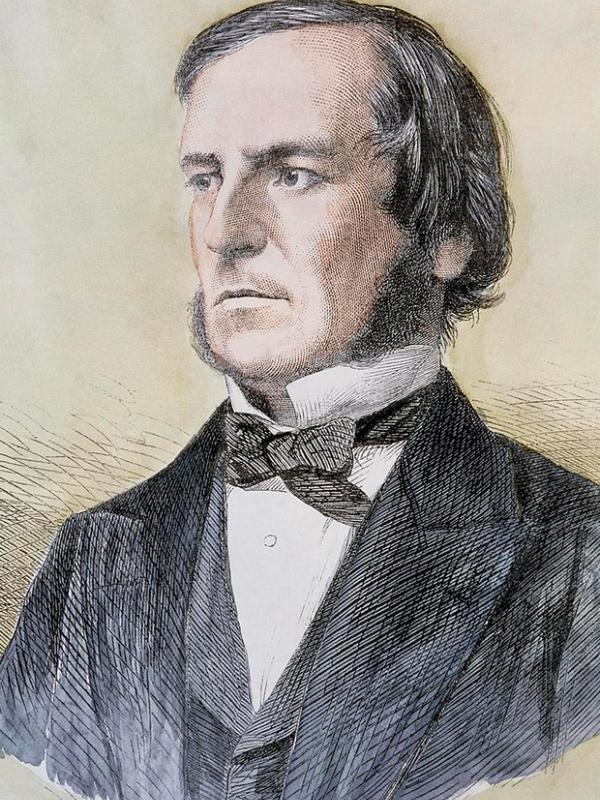
\includegraphics[width=0.9\linewidth]{images/George_Boole_color.jpg}\footnote[frame]{\url{https://commons.wikimedia.org/wiki/File:George_Boole_color.jpg}}
	\end{columns}
\end{frame}

\include{logischer_schluss}
\include{erfuellbarkeit}
\include{einfuehrung_sprachen_grammatiken}
\include{regulaere_sprachen_endliche_automaten}
\include{kellerautomaten}
\section{Kontextfreie Sprachen}

\begin{frame}{Typ-2 Grammatiken: Normalformen}
	\begin{itemize}
		\item Vereinfachungen für kontextfreie Grammatiken $G$
		\begin{itemize}
			\item $\varepsilon$-Regeln eliminieren: $S \rightarrow aAb; A \rightarrow aS|\varepsilon$\\
			wird zu	$S \rightarrow aAb|ab; A \rightarrow aS$
			\item $G$ reduzieren: nutzlose Variablen eliminieren
			\item Kettenregeln $A \rightarrow B$ entfernen
		\end{itemize}
		\item Chomsky-Normalform
		\begin{itemize}
			\item zu jeder $\varepsilon$-freien, reduzierten kontextfreien Grammatik $G$ ohne Kettenregeln lässt sich eine äquivalente Grammatik $G'$ angeben, die nur Regeln der Art $A \rightarrow a$ bzw. $A \rightarrow BC$ enthält.
			\item Konstuktion: Ausgangspunkt $A\rightarrow X_1X_2 \ldots X_m, m\geq 2, X_i \in V \cup \Sigma$
			\begin{itemize}
				\item für $X_i=a\in \Sigma$ neue Variable $X_a$ mit $X_a \rightarrow a$ einführen
				\item verbleibende Regeln $A \rightarrow B_1B_2\ldots B_m, B_i \in V, m\geq 3$:\\
				ersetze $A \rightarrow B_1D_1, D_1\rightarrow B_2D_2, \ldots, D_{m-2}\rightarrow B_{m-1}B_m$ ($D_i$ neue Variablen)
			\end{itemize}
		\end{itemize}
		\item Greibach-Normalform: Regeln vom Typ $A \rightarrow aB_1B_2 \ldots B_m|a$
	\end{itemize}
\end{frame}

\begin{frame}{Beispiel: Erzeugung Chomsky-Normalform}
	$G=(\{S, A, B, C, D, E\}, \{a, b\}, P, S)$\\
	$P=\{$\\
	\qquad\qquad $S \rightarrow bA \mid aB \mid C \mid Cb,$\\
	\qquad\qquad $A \rightarrow bAA \mid aS \mid a \mid bE \mid bDb,$\\
	\qquad\qquad $B \rightarrow aBB \mid bS \mid b,$\\
	\qquad\qquad $C \rightarrow Cc \mid c,$\\
	\qquad\qquad $D \rightarrow d \mid \varepsilon $\\
	\qquad$\}$
\end{frame}

\begin{frame}{Worterkennung: Cocke-Younger-Kasami-Algorithmus (CYK)}
	polynomiell auch für nichtdeterministische Sprachen
	\begin{itemize}
		\item Ziel: Worterkennung und Konstruktion Ableitungsbaum bottom-up
		\item Ausgangspunkt: $G$ in Chomsky-Normalform, $w=a_1a_2 \ldots a_n \in \Sigma^*$
		\item definiere $V[i,j]:=\{A \in V \mid A \underset{G}{\Rightarrow}^* w_{ij} \}$ mit\\
		$w_{ij}=a_ia_{i+1}\ldots a_{i+j-1}, |w_{ij}|=j, 1\leq i \leq n, 1\leq j \leq n+1-i$
		\item es gilt: $w\in L$ gdw. $S \in V[1,n]$
		\item schrittweise Berechnung (Rückführung auf kürzere Teilworte)\\
		$j=1: V[i,1]=\{X \in V \mid (X\rightarrow a_i) \in P\}$\\
		$j>1: V[i,j]=\bigcup_{l=1}^{j-1}\{A\in V\mid \exists (A\rightarrow BC): B \in V[i,l] \land C \in V[i+l, j-l] \}$
		\item Wortproblem mit polynomiellem Zeitaufwand $O(n^3)$ lösbar
		\item Grammatik ist mehrdeutig, falls ein $V[i,j]$ mehrere Einträge hat, die von $S$ aus erreicht werden können
	\end{itemize}
\end{frame}

\begin{frame}{Beispiel: CYK-Algorithmus}
	$$L=\{a^nb^n\mid n\geq 1\}$$
	Zugehörige Grammatik in Chomsky-Normalform:
	\begin{align*}
		G=(&\{A, B, C, S\}, \{a, b\}, P, S)\\
		P=\{&S \rightarrow AB,\\
		    &S \rightarrow AC,\\
		    &C\rightarrow SB,\\
		    &A\rightarrow a,\\
		    &B\rightarrow b\}
	\end{align*}
	
\end{frame}

\note{
	Betrachten des Wortes $w=aabb$\\
	\begin{columns}
		\column{.3\textwidth}
		\begin{itemize}
			\item[$(a)$] $V[1,1]=\{A\}$
			\item[$(a)$] $V[2,1]=\{A\}$
			\item[$(b)$] $V[3,1]=\{B\}$
			\item[$(b)$] $V[4,1]=\{B\}$
			\item[$(aa)$] $V[1,2]=\varnothing$
		\end{itemize}
		\column{.3\textwidth}
		\begin{itemize}
			\item[$(ab)$] $V[2,2]=\{S\}$
			\item[$(bb)$] $V[3,2]=\varnothing$
			\item[$(aab)$] $V[1,3]=\varnothing$
			\item[$(abb)$] $V[2,3]=\{C\} (l=2)$
			\item[$(aabb)$] $V[1,4]=\{S\} (l=1)$
		\end{itemize}
		\column{.4\textwidth}
		\centering
		\begin{tabular}{|c|c|c|c|}
			\hline
			$a$ & $a$ & $b$ & $b$ \\
			\hline
			\hline
			$\{A\}$ & $\{A\}$ & $\{B\}$ & $\{B\}$ \\
			\hline
			$\varnothing$ & $\{S\}$ & $\varnothing$ &  \\
			\hline
			$\varnothing$ & $\{C\}$ &  &  \\
			\hline
			$\{S\}$ &  &  &  \\
			\hline
		\end{tabular}
	\end{columns}
}

\begin{frame}{Pumping-Lemma für kontextfreie Sprachen}
	\begin{itemize}
		\item Pumping-Lemma: für jede kontextfreie Sprache $L$ gilt\\
		es existiert eine natürliche Zahl $n$ so, dass für alle $z \in L$ mit $|z|\geq n$ gilt:\\
		$z$ lässt sich zerlegen in $z=uvwxy$ mit
		\begin{itemize}
			\item $|vx|\geq 1$
			\item $|vwx| \leq n$
			\item $uv^iwx^iy \in L, i=0, 1, 2, \ldots$
		\end{itemize}
		\item Beweis:
		\begin{itemize}
			\item wähle $n=2^m$, $m$: Anzahl der Nichtterminalsymbole, wenn sich G in Chomsky-Normalform befindet
			\item mindestens eine Variable $A$ muss sich im Ableitungsbaum nach spätestens $m$ Schritten wiederholen;\\
			$A\underset{G}{\Rightarrow}^*\omega_1 A \omega_2$, wähle $v: \omega_1 \underset{G}{\Rightarrow}^* v, x: \omega_2 \underset{G}{\Rightarrow}^* x, w: A \underset{G}{\Rightarrow}^* w$;\\
			diese Ableitungen enthalten jeweils keine Wiederholungen von Variablen
		\end{itemize}
	\end{itemize}
\end{frame}

\begin{frame}{Beispiel: Pumping-Lemma für kontextfreie Sprachen}
	$L=\{a^ib^ic^i \mid i\geq 1 \}$
	\begin{itemize}
		\item $L$ ist kontext-sensitiv: Beweis Typ-1-Grammatik\\
		$G=(V, \Sigma, P, S), V=\{S, B, C\}$\\
		$P=\{S\rightarrow aSBC | aBC, CB \rightarrow BC,$\\
		\qquad $aB \rightarrow ab, bB \rightarrow bb, bC \rightarrow bc, cC \rightarrow cc \}$
		\item $L$ ist nicht kontextfrei: Beweis Pumping-Lemma\\
		wäre $L$ kontextfrei, sei $n$ das "`Pumping-$n$"'\\
		wähle $z=a^nb^nc^n \in L, |z|=3n \geq n$\\
		es ex. eine Zerlegung $z=uvwxy$ mit $|vx|\geq 1, |vwx| \leq n$\\
		$\rightarrow$ $vwx$ kann höchstens zwei verschiedene Buchstaben enthalten\\
		$\rightarrow$ in $uv^iwx^iy$ werden ein oder zwei Buchstaben "`aufgepumpt"', der dritte nicht\\
		$\rightarrow$ $uv^iwx^iy \notin L$ für $i \neq 1$ \lightning 
	\end{itemize}
\end{frame}

\begin{frame}{Abschlusseigenschaften kontextfreier Sprachen}
	\begin{itemize}
		\item Kontextfreie Sprachen sind abgeschlossen unter
		\begin{itemize}
			\item Vereinigung: $L_1\cup L_2$\qquad $S \rightarrow S_1|S_2$
			\item Konkatenation: $L_1L_2$ \qquad $S\rightarrow S_1S_2$
			\item Stern-Produkt: $L^*$ \qquad $S_0\rightarrow S|\varepsilon, S\rightarrow S_1|S_1S$
			\item Spiegelung: ersetze in Chomsky-Normalform $A\rightarrow BC$ durch $A \rightarrow CB$
		\end{itemize}
		\item Kontextfreie Sprachen sind \underline{nicht} abgeschlossen unter
		\begin{itemize}
			\item [a)] Durchschnitt\\
			Gegenbeispiel: $L_1=\{a^kb^kc^l\mid k,l\geq 0\}, L_2=\{a^kb^lc^l\mid k,l\geq 0\}$ sind kontextfrei\\
			$L=L_1\cap L_2$ ist nicht kontextfrei
			\item [b)] Komplement\\
			$L_1 \cap L_2 = \overline{\overline{L_1} \cup \overline{L_2}}$: Abgeschlossenheit unter Vereinigung und Komplement würde zu Abgeschlossenheit unter Durchschnitt führen\\
			$\rightarrow$ Widerspruch zu a) \lightning
			
		\end{itemize}
	\end{itemize}
\end{frame}

\begin{frame}{Abschlusseigenschaften deterministisch kontextfreier Sprachen}
	\begin{enumerate}[a)]
		\item Deterministisch kontextfreie Sprachen sind abgeschlossen unter Komplementbildung (beachte: Akzeptanz durch Endzustand!)
		\item Deterministisch kontextfreie Sprachen sind \underline{nicht} abgeschlossen unter
		\begin{enumerate}[i.]
			\item Durchschnitt $L_1 \cap L_2$
			\item Konkatenation $L_1L_2$
			\item Stern-Produkt $L^*$
			\item Vereinigung $L_1 \cup L_2$
		\end{enumerate}
		\item $L_1 \cap L_2$ ist allerdings det. kontextfrei (bzw. kontextfrei) falls $L_1$ regulär und $L_2$ det. kontextfrei (bzw. kontextfrei) ist
	\end{enumerate}
\end{frame}

\include{typ-0-sprachen_turing_maschinen}
\include{abschluss}

\end{document}

